%% Преамбула TeX-файла

% 1. Стиль и язык
\documentclass[utf8x]{G7-32} % Стиль (по умолчанию будет 14pt)
\usepackage[T2A]{fontenc}
\usepackage[russian]{babel}
% Остальные стандартные настройки убраны в preamble.inc.tex.
\sloppy

% Настройки стиля ГОСТ 7-32
% Для начала определяем, хотим мы или нет, чтобы рисунки и таблицы нумеровались в пределах раздела, или нам нужна сквозная нумерация.
\EqInChapter % формулы будут нумероваться в пределах раздела
\TableInChapter % таблицы будут нумероваться в пределах раздела
\PicInChapter % рисунки будут нумероваться в пределах раздела

% Добавляем гипертекстовое оглавление в PDF
\usepackage[
bookmarks=true, colorlinks=true, unicode=true,
urlcolor=black,linkcolor=black, anchorcolor=black,
citecolor=black, menucolor=black, filecolor=black,
]{hyperref}

% Изменение начертания шрифта --- после чего выглядит таймсоподобно.
% apt-get install scalable-cyrfonts-tex

\IfFileExists{cyrtimes.sty}
    {
        \usepackage{cyrtimespatched}
    }
    {
        % А если Times нету, то будет CM...
    }

\usepackage{graphicx}   % Пакет для включения рисунков

% С такими оно полями оно работает по-умолчанию:
% \RequirePackage[left=20mm,right=10mm,top=20mm,bottom=20mm,headsep=0pt]{geometry}
% Если вас тошнит от поля в 10мм --- увеличивайте до 20-ти, ну и про переплёт не забывайте:
\geometry{right=20mm}
\geometry{left=30mm}


% Пакет Tikz
\usepackage{tikz}
\usetikzlibrary{arrows,positioning,shadows}

% Произвольная нумерация списков.
\usepackage{enumerate}

% ячейки в несколько строчек
\usepackage{multirow}

% itemize внутри tabular
\usepackage{paralist,array}


% Настройки листингов.
% 8 Листинги

\usepackage{listings}

% Значения по умолчанию
\lstset{
  basicstyle= \footnotesize,
  breakatwhitespace=true,% разрыв строк только на whitespacce
  breaklines=true,       % переносить длинные строки
%   captionpos=b,          % подписи снизу -- вроде не надо
  inputencoding=koi8-r,
  numbers=left,          % нумерация слева
  numberstyle=\footnotesize,
  showspaces=false,      % показывать пробелы подчеркиваниями -- идиотизм 70-х годов
  showstringspaces=false,
  showtabs=false,        % и табы тоже
  stepnumber=1,
  tabsize=4,              % кому нужны табы по 8 символов?
  frame=single
}

% Стиль для псевдокода: строчки обычно короткие, поэтому размер шрифта побольше
\lstdefinestyle{pseudocode}{
  basicstyle=\small,
  keywordstyle=\color{black}\bfseries\underbar,
  language=Pseudocode,
  numberstyle=\footnotesize,
  commentstyle=\footnotesize\it
}

% Стиль для обычного кода: маленький шрифт
\lstdefinestyle{realcode}{
  basicstyle=\scriptsize,
  numberstyle=\footnotesize
}

% Стиль для коротких кусков обычного кода: средний шрифт
\lstdefinestyle{simplecode}{
  basicstyle=\footnotesize,
  numberstyle=\footnotesize
}

% Стиль для BNF
\lstdefinestyle{grammar}{
  basicstyle=\footnotesize,
  numberstyle=\footnotesize,
  stringstyle=\bfseries\ttfamily,
  language=BNF
}

% Определим свой язык для написания псевдокодов на основе Python
\lstdefinelanguage[]{Pseudocode}[]{Python}{
  morekeywords={each,empty,wait,do},% ключевые слова добавлять сюда
  morecomment=[s]{\{}{\}},% комменты {а-ля Pascal} смотрятся нагляднее
  literate=% а сюда добавлять операторы, которые хотите отображать как мат. символы
    {->}{\ensuremath{$\rightarrow$}~}2%
    {<-}{\ensuremath{$\leftarrow$}~}2%
    {:=}{\ensuremath{$\leftarrow$}~}2%
    {<--}{\ensuremath{$\Longleftarrow$}~}2%
}[keywords,comments]

% Свой язык для задания грамматик в BNF
\lstdefinelanguage[]{BNF}[]{}{
  morekeywords={},
  morecomment=[s]{@}{@},
  morestring=[b]",%
  literate=%
    {->}{\ensuremath{$\rightarrow$}~}2%
    {*}{\ensuremath{$^*$}~}2%
    {+}{\ensuremath{$^+$}~}2%
    {|}{\ensuremath{$|$}~}2%
}[keywords,comments,strings]

% Подписи к листингам на русском языке.
\renewcommand\lstlistingname{\cyr\CYRL\cyri\cyrs\cyrt\cyri\cyrn\cyrg}
\renewcommand\lstlistlistingname{\cyr\CYRL\cyri\cyrs\cyrt\cyri\cyrn\cyrg\cyri}


% Полезные макросы листингов.
% Любимые команды
\newcommand{\Code}[1]{\textbf{#1}}


%For titul
%--------------------------------------
\usepackage{graphicx}
\graphicspath{ {./images/} }
\usepackage{tabularx} % in the preamble
\usepackage[normalem]{ulem}
%--------------------------------------

%graphics
\usepackage{tikz,pgfplots}

\begin{document}

\begin{titlepage}
    \thispagestyle{empty}

    \noindent\begin{minipage}{0.05\textwidth}
        
\includegraphics[scale=0.3]{bmstu}
    \end{minipage}
    \hfill
    \begin{minipage}{0.85\textwidth}\raggedleft
        \begin{center}
            \fontsize{10pt}{0.3\baselineskip}\selectfont \textbf{Министерство науки и высшего образования Российской Федерации \\ Федеральное государственное бюджетное образовательное учреждение \\ высшего образования \\ <<Московский государственный технический университет \\ имени Н. Э. Баумана \\ (национальный исследовательский университет)>> \\ (МГТУ им. Н. Э. Баумана)}
        \end{center}
    \end{minipage}

    \begin{center}
        \fontsize{12pt}{0.1\baselineskip}\selectfont
        \noindent\makebox[\linewidth]{\rule{\textwidth}{4pt}} \makebox[\linewidth]{\rule{\textwidth}{1pt}}
    \end{center}

    \begin{flushleft}
        \fontsize{12pt}{0.8\baselineskip}\selectfont

        ФАКУЛЬТЕТ \uline{
            \hfill
            Информатика и системы управления
            \hfill}

        КАФЕДРА \uline{\mbox{\hspace{4mm}}
            \hfill
            Программное обеспечение ЭВМ и информационные технологии
            \hfill}
    \end{flushleft}

    \vfill
    
    \begin{center}
        \fontsize{19pt}{\baselineskip}\selectfont
        \textbf{Отчет по лабораторной работе № 4} \\
        \textbf{по курсу "Анализ алгоритмов"}
    \end{center}

    \vfill
    
    \begin{flushleft}
        Студент \uline{\hfill Недолужко Денис Вадимович \hfill}
        
        Группа \uline{\hfill ИУ7-53Б \hfill}
        
        Название предприятия \uline{\hfill МГТУ им. Н. Э. Баумана, каф. ИУ7  \hfill}
        
        Тема \uline{\hfill Параллельное лексикографическое сравнение строк \hfill}
    \end{flushleft}
    
    \vfill
    
    \begin{flushleft}
    \begin{tabularx}{\textwidth}{Xcc}
      Студент& \uline{\hfill} &  \hfill\uline{Недолужко Д. В.}\\
      &\textsuperscript{\scriptsize{(Подпись, дата)}}&\textsuperscript{\scriptsize{(И.О. Фамилия)}}\\
      Руководитель курсовой работы & \uline{\hfill} & \uline{Волкова Л. Л.}\\
      &\textsuperscript{\scriptsize{(Подпись, дата)}}&\textsuperscript{\scriptsize{(И.О. Фамилия)}}\\
    \end{tabularx}
    \end{flushleft}
    
    \vfill
    
    \begin{center}
        \normalsize Москва \\
        \the\year ~г.
    \end{center}
\end{titlepage}

\frontmatter % выключает нумерацию ВСЕГО; здесь начинаются ненумерованные главы: реферат, введение, глоссарий, сокращения и прочее.

% Команды \breakingbeforechapters и \nonbreakingbeforechapters
% управляют разрывом страницы перед главами.
% По-умолчанию страница разрывается.

% \nobreakingbeforechapters
% \breakingbeforechapters


\mainmatter % это включает нумерацию глав и секций в документе ниже

\tableofcontents

\chapter*{Введение}
\addcontentsline{toc}{chapter}{Введение}

Расстояние Левенштейна (редакционное расстояние, дистанция редактирования) — метрика, измеряющая по модулю разность между двумя последовательностями символов. Она определяется как минимальное количество односимвольных операций (а именно вставки, удаления, замены), необходимых для превращения одной последовательности символов в другую. В общем случае, операциям, используемым в этом преобразовании, можно назначить разные цены. Широко используется в теории информации и компьютерной лингвистике.

Впервые задачу поставил в 1965 году советский математик Владимир Левенштейн при изучении последовательностей \(0 − 1\) \cite{leven1965}, впоследствии более общую задачу для произвольного алфавита связали с его именем.

Расстояние Левентшейна используется:

\begin{itemize}
    \item в компьютерной лингвистике для проведения автозамены
    \item в биоинформатике для сравнения генов, хромосом, белков
    \item в утилите diff для определения изменений в текстовых файлов
\end{itemize}

Расстояние Дамерау — Левенштейна (названо в честь учёных Фредерика Дамерау и Владимира Левенштейна) — это мера разницы двух строк символов, определяемая как минимальное количество операций вставки, удаления, замены и транспозиции (перестановки двух соседних символов), необходимых для перевода одной строки в другую. Является модификацией расстояния Левенштейна: к операциям вставки, удаления и замены символов, определённых в расстоянии Левенштейна добавлена операция транспозиции (перестановки) символов.

Целью работы является исследование алгоритмов Левенштейна и Дамераy - Левенштейна.

Для достижения поставленной цели необходимо выполнить следующие задачи:

\begin{enumerate}
    \item изучение алгоритма Левенштейна и Демаран - Левенштейна
    \item реализация рекурсивных (без кеша) и итеративных (с кешем) алгоритмов Левенштейна и Дамераy - Левенштейна
    \item замер и сравнение процессорного времени затрачиваемых реализованными алгоритмами
    \item замер и сравнение используемой памяти реализованными алгоритмами
\end{enumerate}
\chapter{Аналитическая часть}

    В данном разделе описаны математические модели исследуемой области.

    \section{Расстояние Левенштейна}

    Расстояние редакционное, расстояние Левеншейна - это минимальное
    количество операций, необходимое для превращений одной строки в другую.
    
    Для определения стоимости преобразований вводятся следующие операции
    со величиной штрафа - 1:
    
    \begin{itemize}
        \item I (от англ. insert) - вставка
        \item D (от англ. delete) - удаление
        \item R (от англ. replace) - замена
    \end{itemize}
    
    Также вводится обозначение М (от англ. match). Штраф для совпадении двух
    символом считается равным 0.
    
    \section{Рекурсивный алгоритм нахождения расстояния Левенштейна}
        
        Расстояние Левенштейна между двумя строками a и b может быть вычислено по формуле \ref{eq:D}, где $|a|$ означает длину строки $a$; $a[i]$ — i-ый символ строки $a$ , функция $D(i, j)$ определена как:
        \begin{equation}
        	\label{eq:D}
        	D(i, j) = \begin{cases}
        		0 &\text{i = 0, j = 0}\\
        		i &\text{j = 0, i > 0}\\
        		j &\text{i = 0, j > 0}\\
        		\min \lbrace \\
        			\qquad D(i, j-1) + 1\\
        			\qquad D(i-1, j) + 1 &\text{i > 0, j > 0}\\
        			\qquad D(i-1, j-1) + m(a[i], b[j]) &\text(\ref{eq:m})\\
        		\rbrace
        	\end{cases},
        \end{equation}
        
        а функция \ref{eq:m} определена как:
        \begin{equation}
        	\label{eq:m}
        	m(a, b) = \begin{cases}
        		0 &\text{если a = b,}\\
        		1 &\text{иначе}
        	\end{cases}.
        \end{equation}
        
        Рекурсивный алгоритм реализует формулу \ref{eq:D}.
        Функция $D$ составлена из следующих соображений:
        \begin{enumerate}
        	\item для перевода из пустой строки в пустую требуется ноль операций;
        	\item для перевода из пустой строки в строку $a$ требуется $|a|$ операций;
        	\item для перевода из строки $a$ в пустую требуется $|a|$ операций;
        \end{enumerate}
        Для перевода из строки $a$ в строку $b$ требуется выполнить последовательно некоторое количество операций (удаление, вставка, замена) в некоторой последовательности. Последовательность проведения любых двух операций можно поменять, порядок проведения операций не имеет никакого значения. Полагая, что $a', b'$  — строки $a$ и $b$ без последнего символа соответственно, цена преобразования из строки $a$ в строку $b$ может быть выражена как:
        	\begin{enumerate}
        		\item сумма цены преобразования строки $a$ в $b$ и цены проведения операции удаления, которая необходима для преобразования $a'$ в $a$;
        		\item сумма цены преобразования строки $a$ в $b$  и цены проведения операции вставки, которая необходима для преобразования $b'$ в $b$;
        		\item сумма цены преобразования из $a'$ в $b'$ и операции замены, предполагая, что $a$ и $b$ оканчиваются разные символы;
        		\item цена преобразования из $a'$ в $b'$, предполагая, что $a$ и $b$ оканчиваются на один и тот же символ.
        	\end{enumerate}
        Минимальной ценой преобразования будет минимальное значение приведенных вариантов.
    
    \section{Матричный алгоритм нахождения расстояния Левенштейна}
    
        Прямая реализация формулы \ref{eq:D} может быть малоэффективна по времени исполнения при больших $i, j$, т. к. множество промежуточных значений $D(i, j)$ вычисляются заново множество раз подряд. Для оптимизации нахождения расстояния Левенштейна можно использовать матрицу в целях хранения соответствующих промежуточных значений. В таком случае алгоритм представляет собой построчное заполнение матрицы 
        $A_{|a|,|b|}$ значениями $D(i, j)$.
    
    \section{Рекурсивный алгоритм нахождения расстояния Левенштейна с заполнением матрицы}
        \label{sec:recmat}
        
        Рекурсивный алгоритм заполнения можно оптимизировать по времени выполнения с использованием матричного алгоритма. Суть данного метода заключается в параллельном заполнении матрицы при выполнении рекурсии. В случае, если рекурсивный алгоритм выполняет прогон для данных, которые еще не были обработаны, результат нахождения расстояния заносится в матрицу. В случае, если обработанные ранее данные встречаются снова, для них расстояние не находится и алгоритм переходит к следующему шагу.
    
    \section{Расстояния Дамерау — Левенштейна}
    
        Расстояние Дамерау — Левенштейна может быть найдено по формуле \ref{eq:d}, которая задана как
        \begin{equation}
        	\label{eq:d}
        	d_{a,b}(i, j) = \begin{cases}
        		\max(i, j), &\text{если }\min(i, j) = 0,\\
        		\min \lbrace \      \
        			\qquad d_{a,b}(i, j-1) + 1,\\
        			\qquad d_{a,b}(i-1, j) + 1, &\text{иначе}\\
        			\qquad d_{a,b}(i-1, j-1) + m(a[i], b[j]),\\
        			\qquad \left[ \begin{array}{cc}d_{a,b}(i-2, j-2) + 1, &\text{если }i,j > 1;\\
        			\qquad &\text{}a[i] = b[j-1]; \\
        			\qquad &\text{}b[j] = a[i-1]\\
        			\qquad \infty, & \text{иначе}\end{array}\right.\\
        		\rbrace
        		\end{cases},
        \end{equation}
        
        Формула выводится по тем же соображениям, что и формула (\ref{eq:D}).
        Как и в случае с рекурсивным методом, прямое применение этой формулы неэффективно по времени исполнения, то аналогично методу из \ref{sec:recmat} производится добавление матрицы для хранения промежуточных значений рекурсивной формулы.
    
    \section*{Вывод}
    \addcontentsline{toc}{section}{Вывод}
    
        В результате были рассмотрены и описаны математические модели следующих алгоритмов:
        
        \begin{itemize}
            \item Рекурсивный алгоритм нахождения расстояния Левенштейна
            \item Mатричный алгоритм нахождения расстояния Левенштейна
            \item Рекурсивный алгоритм нахождения расстояния Дамерау - Левенштейна
            \item Mатричный алгоритм нахождения расстояния Дамерау - Левенштейна
        \end{itemize}
        
        В качестве входных данных алгоритмы принимают 2 строки, по которым рассчитывается искомое расстояние. Выходными данными алгоритма является число - найденное расстояние.
        
        Ограничением для реализуемой программы является обработка строк только в кодах ascii.c
\chapter{Конструкторская часть}
    
    \section{Блок схемы алгоритмов}
    
        \begin{figure}
            \centering
            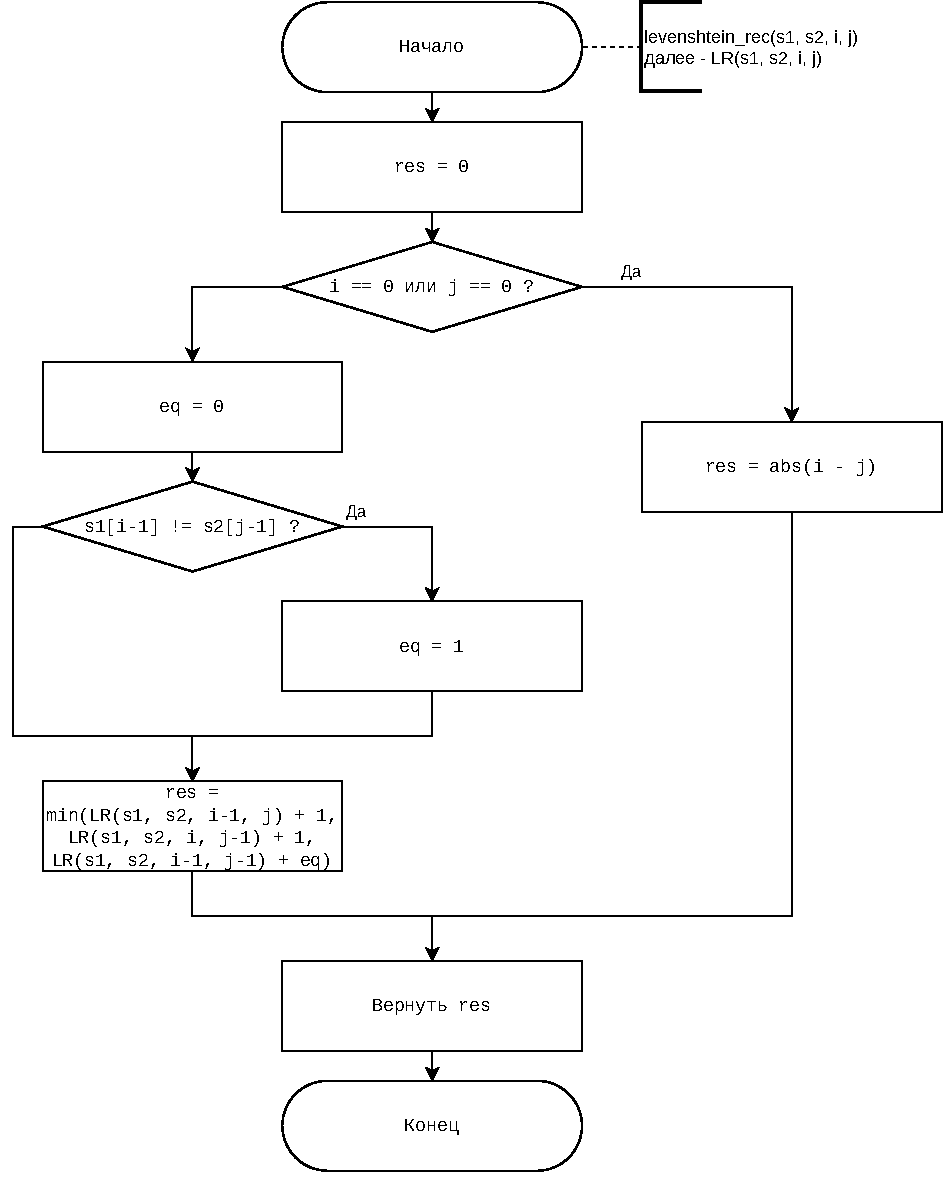
\includegraphics[width=15cm,height=25cm,keepaspectratio]{images/leven_rec.pdf}
            \caption{Рекурсивный алгоритм Левенштейна}
            \label{fig:leven_rec}
        \end{figure}
        
        \begin{figure}
            \centering
            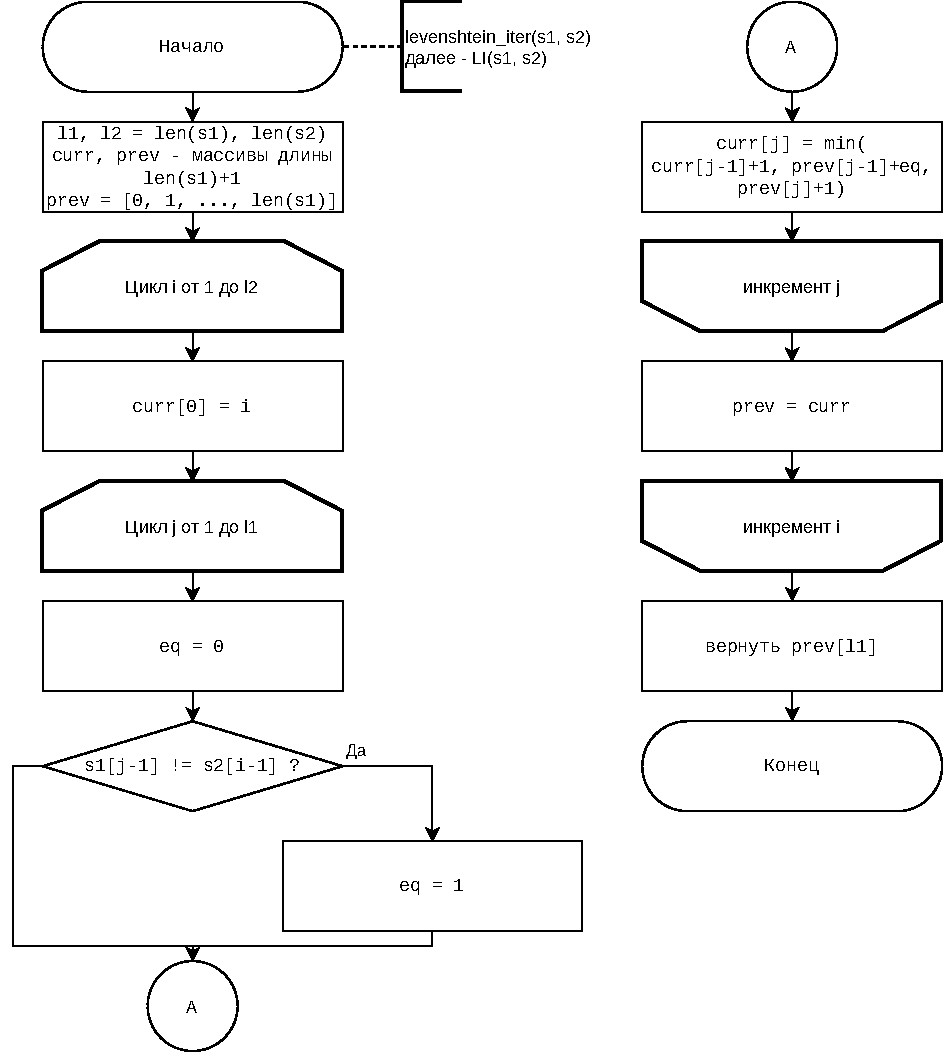
\includegraphics[width=15cm,height=25cm,keepaspectratio]{images/leven_iter.pdf}
            \caption{Рекурсивный алгоритм Левенштейна}
            \label{fig:leven_iter}
        \end{figure}
        
        \begin{figure}
            \centering
            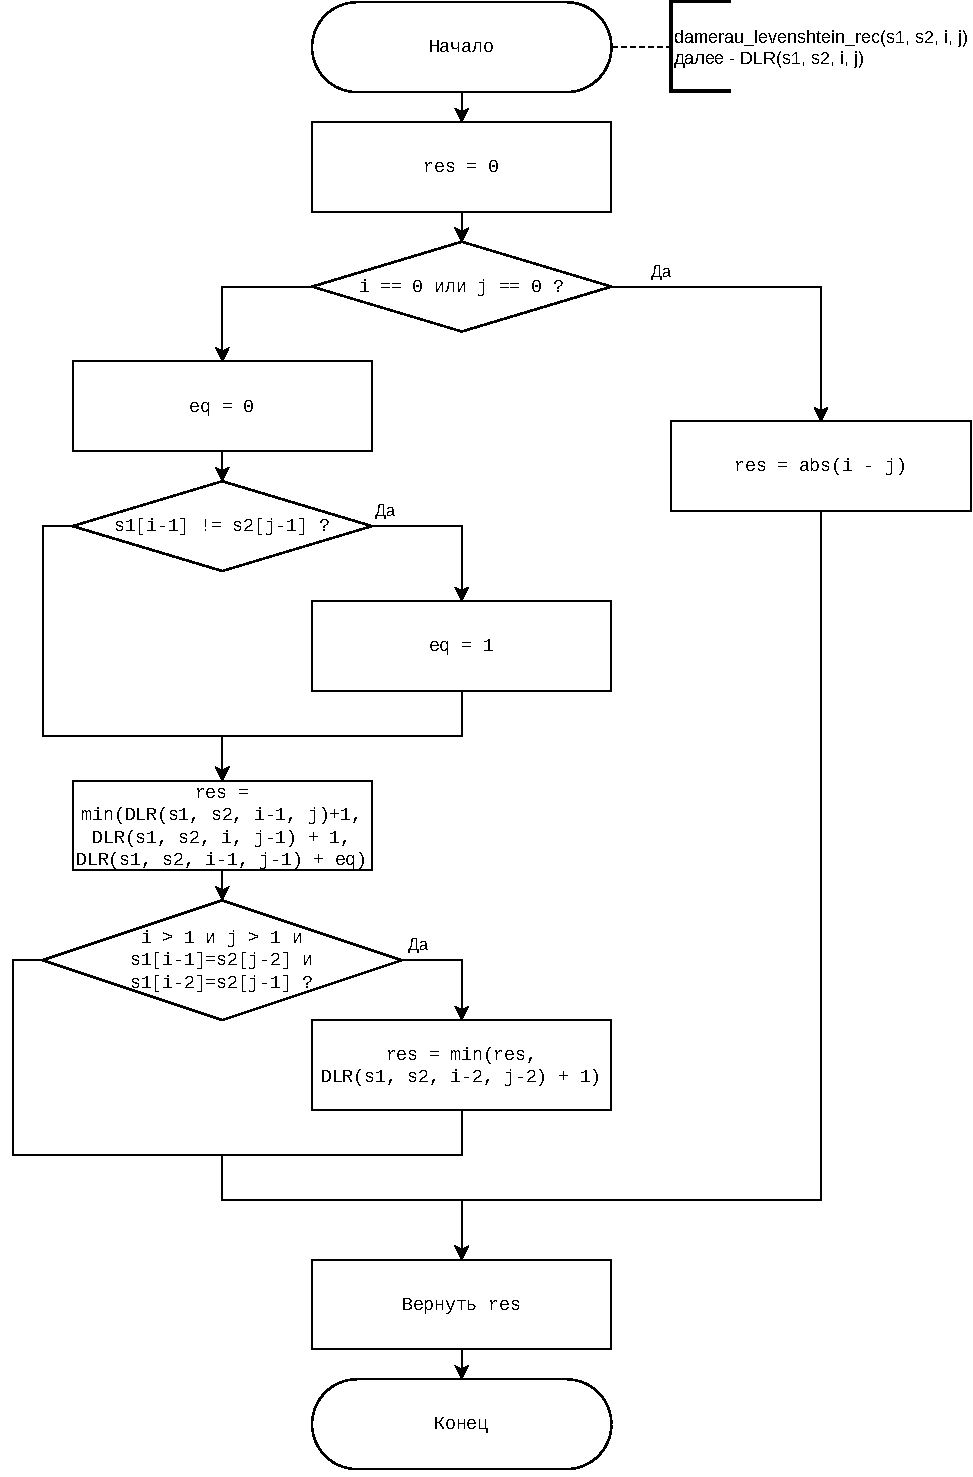
\includegraphics[width=15cm,height=25cm,keepaspectratio]{images/dleven_rec.pdf}
            \caption{Итеративный алгоритм Дамерау - Левенштейна}
            \label{fig:dleven_rec}
        \end{figure}
        
        \begin{figure}
            \centering
            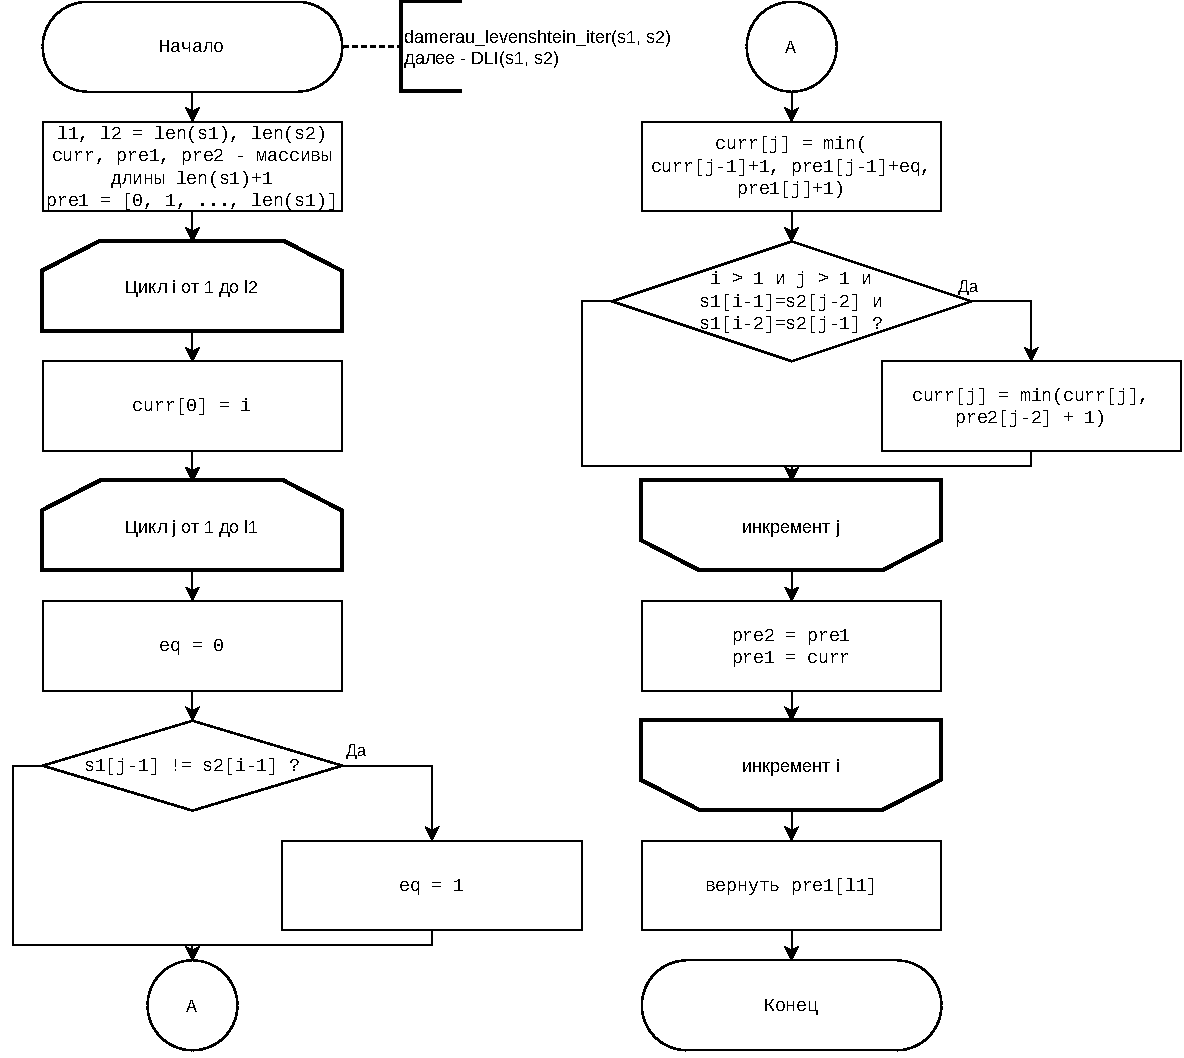
\includegraphics[width=15cm,height=25cm,keepaspectratio]{images/dleven_iter.pdf}
            \caption{Рекурсивный алгоритм Дамерау - Левенштейна}
            \label{fig:dleven_iter}
        \end{figure}
    
    \clearpage

    \section*{Вывод}
    \addcontentsline{toc}{section}{Вывод}
    
        На основе теоретических данных, полученных из аналитического раздела были построены схемы требуемых алгоритмов.
\chapter{Технологическая часть}

    В данном разделе приведены требования к программному обеспечению, средства реализации и листинги кода.
    
    \section{Выбор средств реализации}
        
        Для реализации библиотеки с реализациями алгоритмов мною был выбрал язык C стандарта 1999 года. Он был выбран в силу отсутствия необходимости в использовании высокоуровневых абстракций.
        
        Для реализации клиента был выбран язык C расширения GNU 99 года, так как он предоставляет фукнкции чтения динамических строк.
        
        Для юнит тестирования был выбран язык C++14, для использовая фрейворка GoogleTests\cite{gtests}.
    
    \section{Требования к программному обеспечению}
    
        К программе предъявляется ряд требований:
        
        \begin{itemize}
            \item На вход подаётся две регистрозависимые строки.
            \item На выходе — результат выполнения каждого из вышеуказанных алгоритмов.
        \end{itemize}
    
    \clearpage
    
    \section{Листинги кода}
    
        \lstinputlisting[
        language={C},
        caption=Основной файл программы main.c,
        basicstyle=\scriptsize
        ]{./listings/main.c}
        
        \clearpage
        
        \lstinputlisting[
        language={C},
        caption=Рекурсивная функция нахождения расстояния Левенштейна,
        basicstyle=\scriptsize
        ]{./listings/leven_rec.c}
        
        \lstinputlisting[
        language={C},
        caption=Рекурсивная функция нахождения расстояния Дамерау - Левенштейна,
        basicstyle=\scriptsize
        ]{./listings/dleven_rec.c}
        
        \lstinputlisting[
        language={C},
        caption=Итеративная функция нахождения расстояния Левенштейна,
        basicstyle=\scriptsize
        ]{./listings/leven_iter.c}
        
        \clearpage
        
        \lstinputlisting[
        language={C},
        caption=Итеративная функция нахождения расстояния Дамерау - Левенштейна,
        basicstyle=\scriptsize
        ]{./listings/dleven_iter.c}
        
        \clearpage
        
        \lstinputlisting[
        language={C},
        caption=Вспомогательные функции,
        basicstyle=\scriptsize
        ]{./listings/support.c}
        
    \section*{Вывод}
    \addcontentsline{toc}{section}{Вывод}
    
        Были реализованы алгоритмы: вычисления расстояния Левенштейна рекурсивно, с зaполнением кэша, а также вычисления расстояния Дамерау – Левенштейна рекурсивно и вычисления расстояния Дамерау – Левенштейна с заполнением кэша.
\chapter{Экспериментальная часть}

    В данном разделе будет проведено функциональное тестирование разработанного программного обеспечения. Так же будет произведено измерение временных характеристик и характеристик по памяти каждого из реализованных алгоритмов.

    \section{Технические характеристики}
    
        Технические характеристики устройства, на котором выполнялось исследование:
        
        \begin{itemize}
            \item Процессор: Intel(R) Core(TM) i5-8250U CPU @ 1.60GHz \cite{intel}
            \item Оперативная память: 8 Gb
            \item Операционная система: elementary OS 6 Odin \cite{elemos}
        \end{itemize}
    
    \section{Тестирование}
    
        Юнит тестирование проводилось при помощи фрэймворка GoogleTests. Были выполнены следующие тесты
        
        \begin{table}[]
            \centering
            \caption{Функциональные тесты}
            \begin{tabular}{|c|c|c|c|}
\hline \textbf{Строка 1} & \textbf{Строка 2} & \textbf{Левенштейн} & \textbf{Дамерау-Левенштейн}  \\
\hline CONNECT & CONEHEAD & 4 &  \\
\hline & CONEHEAD & 8 & 8 \\
\hline &  & 0 & 0 \\
\hline deniska & deniska & 0 & 0 \\
\hline abc & bc & 1 & 1 \\
\hline abc & ac & 1 & 1 \\
\hline abc & ab & 1 & 1 \\
\hline abc & xbc & 1 & 1 \\
\hline abc & axc & 1 & 1 \\
\hline abc & abx & 1 & 1 \\
\hline CONNECT & CNNNETC &  & 2 \\
\hline abcd & badc &  & 2 \\
\hline
            \end{tabular}
            \label{tab:my_label}
        \end{table}
        
        
        При проведении функционального тестирования, полученные результаты работы программы совпали с ожидаемыми. Таким образом, функциональное тестирование пройдено успешно.
    
    \section{Временные характеристики}
    
        Результаты замеров по результатам экспериментов приведены в Таблице \ref{tab:time}. В данной таблице для значений, для которых тестирование не выполнялось, в поле результата находится ” - ”.
    
        \begin{table}[]
            \centering
            \caption{Замер времени для строк разной длины}
            \resizebox{\columnwidth}{!}{% 
            \begin{tabular}{|c|c|c|c|c|}
\hline \multirow{3}{*}{\textbf{Длина строк}} & \multicolumn{4}{c|}{\textbf{Время, сек}} \\
\cline{2-5} & \multicolumn{2}{c|}{\textbf{Левенштейн}} & \multicolumn{2}{c|}{\textbf{Дамерау-Левенштейн}} \\
\cline{2-5} & \textbf{Рекурсивный} & \textbf{Итеративный} & \textbf{Рекурсивный} & \textbf{Итеративный} \\
\hline    1 &   3e-08 & 5.3e-08 & 3.6e-08 & 6.6e-08 \\
\hline    2 & 6.7e-05 & 3.1e-07 & 6.6e-05 & 3.8e-07 \\
\hline    4 & 8.1e-05 & 3.2e-07 & 6.6e-05 & 3.8e-07 \\
\hline    6 & 6.6e-04 & 4.2e-07 & 6.5e-05 & 3.8e-07 \\
\hline    8 &  0.0019 & 5.2e-07 &   0.002 & 6.7e-07 \\
\hline   16 &       - &   2e-06 &       - & 2.7e-06 \\
\hline   32 &       - & 8.8e-06 &       - & 1.3e-05 \\
\hline   64 &       - & 3.5e-05 &       - & 4.4e-05 \\
\hline  128 &       - & 0.00012 &       - & 0.00016 \\
\hline  256 &       - & 0.00048 &       - & 0.00064 \\
\hline  512 &       - &  0.0019 &       - &  0.0025 \\
\hline 1024 &       - &  0.0075 &       - &    0.01 \\
\hline
            \end{tabular}%
            }
            \label{tab:time}
        \end{table}
    
   Отдельно сравним итеративные алгоритмы поиска расстояний Левенштейна и Дамерау– Левенштейна. Сравнение будет производится на основе данных, представленных в Таблице \ref{tab:time}. Результат можно увидеть на Рисунке \ref{plt:time_cmp_l_dl}. 
        
    \begin{figure}[!h]
      \centering
      \begin{tikzpicture}
        \begin{axis}[
          axis lines=left,
          xlabel=Длина строк,
          ylabel={Время, мс},
          legend pos=north west,
          ymajorgrids=true
        ]
          \addplot table[x=strlen,y=leven_iter,col sep=comma] {datasheets/itr.csv};
          \addplot table[x=strlen,y=dleven_iter,col sep=comma] {datasheets/itr.csv};
          \legend{Левенштейн, Дамерау-Левенштейн}
        \end{axis}
      \end{tikzpicture}
      \captionsetup{justification=centering}
      \caption{Сравнение времени работы итеративных алгоритмов Левенштейна и Дамерау-Левенштейна}
      \label{plt:time_cmp_l_dl}
    \end{figure}
    
    При длинах строк менее 64 символов разница по времени между итеративными реализациями незначительна, однако при увеличении длины строки алгоритм поиска расстояния Левенштейна оказывается быстрее вплоть до полутора раз. Это обосновывается тем, что у алгоритма поиска расстояния Дамерау-Левенштейна задействуется дополнительная операция, которая замедляет алгоритм.
    
    Так же сравним рекурсивную и итеративную реализации алгоритма поиска расстояния Левенштейна. Данные представлены в Таблице \ref{tab:time} и отображены на Рисунке \ref{plt:time_cmp_rec_iter}.
   
    \begin{figure}[!h!]
      \centering
      \begin{tikzpicture}
        \begin{axis}[
          axis lines=left,
          xlabel=Длина строк,
          ylabel={Время, мс},
          legend pos=north west,
          ymajorgrids=true
        ]
          \addplot table[x=strlen,y=leven_rec,col sep=comma] {datasheets/all.csv};
          \addplot table[x=strlen,y=leven_iter,col sep=comma] {datasheets/all.csv};
          \legend{Рекурсивный, Итеративный}
        \end{axis}
      \end{tikzpicture}
      \captionsetup{justification=centering}
      \caption{Сравнение времени работы итеративного и рекурсивного алгоритмов Леверштейна}
      \label{plt:time_cmp_rec_iter}
    \end{figure}
    
    \clearpage
    
    \section{Характеристики по памяти}
    
        Алгоритмы Левенштейна и Дамерау — Левенштейна не отличаются друг от друга с точки зрения использования памяти, следовательно, достаточно рассмотреть лишь разницу рекурсивной и матричной реализаций этих алгоритмов.
        
        Максимальная глубина стека вызовов при рекурсивной реализации равна сумме длин входящих строк, соответственно, максимальный расход памяти (\ref{for:99})
        \begin{equation}
        (\mathcal{C}(S_1) + \mathcal{C}(S_2)) \cdot (2 \cdot \mathcal{C}\mathrm{(string)} + 3 \cdot \mathcal{C}\mathrm{(int)}),
        \label{for:99}
        \end{equation}
        где $\mathcal{C}$ — оператор вычисления размера, $S_1$, $S_2$ — строки, $\mathrm{int}$ — целочисленный тип, $\mathrm{string}$ — строковый тип.
        
        Использование памяти при итеративной реализации теоретически равно
        \begin{equation}
        (\mathcal{C}(S_1) + 1) \cdot (\mathcal{C}(S_2) + 1) \cdot \mathcal{C}\mathrm{(int)} + 10\cdot \mathcal{C}\mathrm{(int)} + 2 \cdot \mathcal{C}\mathrm{(string)}.
        \end{equation}
        
    \section{Сравнительный анализ алгоритмов}
    
        Приведенные характеристики показывают нам, что рекурсивная реализация алгоритма очень сильно проигрывает по времени. В связи с этим, рекурсивные алгоритмы следует использовать лишь для малых размерностей строк (1-2 символа) или при малом объеме оперативной памяти.
        
        Так как во время печати очень часто возникают ошибки связанные с транспозицией букв, алгоритм поиска расстояния Дамерау – Левенштейна является наиболее предпочтительным, не смотря на то, что он проигрывает по времени и памяти алгоритму Левенштейна.
        
        По аналогии с первым абзацем можно сделать вывод о том, что рекуррентный алгоритм поиска расстояния Дамерау - Левенштейна будет более затратным по времени по сравнению с итеративной реализацией алгоритма поиска расстояния Дамерау – Левенштейна с кешированием.
    
    \section*{Вывод}
    \addcontentsline{toc}{section}{Вывод}
    
        В данном разделе было произведено сравнение количества затраченного времени и пaмяти вышеизложенных алгоритмов. Наименее затратным по времени оказался рекурсивный алгоритм нахождения расстояния Дамерау – Левенштейна.
        
        Для обработок малых длин строк (1 – 2 символа) предпочтительнее использовать рекурсивные алгоритмы, в то время как для остальных случаев рекомендуются использовать итеративные реализации. Однако, стоит учитывать дополнительные затраты по памяти, возникающие при использовании итеративных алгоритмов.
\chapter*{Заключение}
\addcontentsline{toc}{chapter}{Заключение}

    В результате выполнения данной лабораторной рабоыт были изучены алгоритмы лексикографического сравнения строк, построены схемы алгоритмов, реализованы данных алгоритмы и проведено их сравнение.
    
    Паралельный алгоритм лексикографиеческого сравнения строк для количестве потоков равном количеству ядер процессора в среднем работает быстрее последовательного в 4-5 раз. Наибольшим выигрыш наблюдается при числе потоков равном максимальному числу потоков, которые могут физически выполнять одновременно. Дальнейнее увеличение числа потоков к росту производительности не ведет.
\renewcommand\bibname{Список литературы}
\bibliographystyle{gost780u}
\bibliography{main.bib}

\end{document}

%%% Local Variables:
%%% mode: latex
%%% TeX-master: t
%%% End:
